% =====================================================================
% Fukuoka talk deck — IEEE BigDataService 2026, Special Track on Secure AI.
% Restyled 2026-07-25: flat theme, ColorBrewer-derived palette (validated
% for CVD separation and surface contrast), peer-review fixes applied
% (instantiation caveats, bar-binding framing, idiom cleanup, backup
% section). Main flow = frames 1-14 (18-minute plan); backups after
% \appendix. The PPTX twin is build_pptx.py — keep them in sync.
% =====================================================================
\documentclass[aspectratio=169,11pt]{beamer}

% ---- Flat theme ------------------------------------------------------
\usetheme{default}
\usepackage[T1]{fontenc}
\usepackage{lmodern}
\usepackage{helvet}
\renewcommand{\familydefault}{\sfdefault}
\usepackage{booktabs}
\usepackage{graphicx}
\usepackage{tikz}
\usepackage{pgfplots}
\pgfplotsset{compat=1.17}
\graphicspath{{revision/assets/}}

% ColorBrewer-derived palette (validated: CVD ΔE and 3:1 surface contrast)
\definecolor{cbblue}{HTML}{2171B5}   % Blues — structure / general factor
\definecolor{cborange}{HTML}{D95F02} % Dark2 orange — accent / specific
\definecolor{cbteal}{HTML}{1B9E77}   % Dark2 teal — mixed / defended
\definecolor{ink}{HTML}{1A2340}
\definecolor{cbgray}{HTML}{636363}

\setbeamercolor{normal text}{fg=ink}
\setbeamercolor{structure}{fg=cbblue}
\setbeamercolor{frametitle}{fg=ink,bg=}
\setbeamercolor{title}{fg=ink}
\setbeamercolor{block title}{fg=cbblue,bg=cbblue!8}
\setbeamercolor{block body}{fg=ink,bg=cbblue!4}
\setbeamercolor{alerted text}{fg=cborange}
\setbeamerfont{frametitle}{series=\bfseries,size=\large}
\setbeamerfont{title}{series=\bfseries,size=\LARGE}
\setbeamertemplate{navigation symbols}{}
\setbeamertemplate{caption}{\insertcaption}
\setbeamertemplate{itemize item}{\textcolor{cbblue}{\scriptsize$\blacksquare$}}
\setbeamertemplate{itemize subitem}{\textcolor{cbgray}{--}}

% flat frametitle: ink title over a thin blue rule
\setbeamertemplate{frametitle}{%
  \vskip1.2ex
  {\usebeamerfont{frametitle}\usebeamercolor[fg]{frametitle}\insertframetitle}\par
  \vskip0.6ex
  {\color{cbblue}\rule{\textwidth}{0.9pt}}\vskip0.4ex}

% minimal footline: short title · venue · frame number (no total, so the
% backup section does not distort the count)
\setbeamertemplate{footline}{%
  \vskip2pt
  \hbox{\hskip4mm{\color{cbgray}\tiny\insertshorttitle\ \ \textperiodcentered\ \
  IEEE BigDataService 2026, Fukuoka}\hfill
  {\color{cbgray}\tiny\insertframenumber}\hskip4mm}\vskip3pt}

% left-rule block flavor for emphasis boxes
\newenvironment{ruledblock}[1]{%
  \begin{beamercolorbox}[sep=6pt,rounded=false]{block body}%
  {\color{cbblue}\textbf{#1}}\par\smallskip}{\end{beamercolorbox}}

\newcommand{\hi}[1]{\textcolor{cbblue}{\textbf{#1}}}
\newcommand{\gold}[1]{\textcolor{cborange}{\textbf{#1}}}

\title[Selective Invariance Violations]{Selective Invariance Violations in\\Large Language Model Moral Judgment}
\subtitle{A Geometric Framework for Behavioral Manipulation Detection}
\author[A.\,H.\,Bond]{Andrew H. Bond}
\institute[SJSU]{Dept.\ of Computer Engineering, San Jose State University}
\date{IEEE BigDataService 2026 --- Special Track on Secure AI}
\titlegraphic{
\includegraphics[height=1.8cm]{atlas_mark_light.pdf}}

\begin{document}

{\setbeamertemplate{footline}{}\begin{frame}\titlepage\end{frame}}

% ---------------------------------------------------------------
\begin{frame}{The problem: LLMs as decision services}
\begin{itemize}
  \item LLMs increasingly gate \hi{safety-critical decisions} --- content moderation, clinical triage, legal analysis.
  \item A secure evaluator should judge the \hi{facts}, not their \hi{presentation}.
  \item \alert{Behavioral manipulation vulnerability}: an attacker shifts the decision by changing morally \emph{irrelevant} surface features --- framing, tone, sensory detail --- without changing the underlying situation.
\end{itemize}
\vfill
\begin{block}{The measurement gap}
Prior work probes one bias at a time and reports a \hi{single scalar robustness score}. Across $n$ independent failure directions, a scalar discards $n-1$ of them. \gold{No post-hoc procedure recovers the lost structure.}
\end{block}
\end{frame}

% ---------------------------------------------------------------
\begin{frame}{Our approach: a geometric vulnerability profile}
\begin{columns}[T]
\begin{column}{0.62\textwidth}
\begin{itemize}
  \item Map each judgment to a point in a \hi{7-D harm space}\\
  {\small (physical, emotional, financial, autonomy, trust, social, identity; each 0--10).}
  \item Apply qualitatively distinct \hi{perturbations}; measure \hi{displacement} of the judgment vector.
  \item Output a \hi{per-model vulnerability profile}, not one number.
  \item Runs under a realistic \hi{\$50/day} compute budget.
\end{itemize}
\end{column}
\begin{column}{0.36\textwidth}
\centering

\includegraphics[height=2.6cm]{erisml_apple_light.pdf}\\[2pt]
{\scriptsize The 7-D space is a measurement-reliable projection of the \hi{DEME v3} 9-D moral vector\\(correspondence table in backup).}
\end{column}
\end{columns}
\end{frame}

% ---------------------------------------------------------------
\begin{frame}{Finding 1 --- Vulnerabilities are \emph{selective}}
\begin{columns}[T]
\begin{column}{0.5\textwidth}
\textbf{Displace judgments (real attack surface):}
\begin{itemize}
  \item \gold{Linguistic framing}
  \item \gold{Emotional anchoring} ($d_z=0.60$--$1.06$)
  \item \gold{Irrelevant sensory detail}
\end{itemize}
\textbf{Do \emph{not} displace:}
\begin{itemize}
  \item Gender swap
  \item Evaluation order
\end{itemize}
\end{column}
\begin{column}{0.5\textwidth}
\begin{block}{The common thread}
The three live surfaces all make morally irrelevant features \hi{perceptually salient}.\\[4pt]
$\Rightarrow$ The attack mechanism is \gold{salience manipulation} --- and the framework discriminates it from noise.
\end{block}
\end{column}
\end{columns}
\vfill
{\small We lead with \hi{effect sizes} (paired $d_z$, displacement in harm-points) over $\sigma$; empirical control arms rule out stochastic drift.}
\end{frame}

% ---------------------------------------------------------------
\begin{frame}{Finding 2 --- Robustness profiles are dissociable}
\begin{itemize}
  \item \hi{No model dominates} all attack surfaces.
  \item Claude: \gold{zero observed sycophancy} (0/9) --- but \gold{worst} emotional-anchoring recovery (20\%) and worst divided attention.
  \item Flash 2.0: \gold{best} anchoring recovery (73\%) --- but \gold{worst} working memory.
\end{itemize}
\vfill
\begin{block}{Consequence for Secure AI}
Averaging partially-independent dimensions yields a number that \alert{describes no model accurately.}\\
\gold{Single-test certification provides false assurance.}
\end{block}
\end{frame}

% ---------------------------------------------------------------
\begin{frame}{Validation (reviewer-driven) --- is the harm space measurable?}
\textbf{Is the 7-D space reliably measurable, or asserted?}\\[2pt]
Inter-model agreement over an \hi{open, multi-family panel} (6 models, 5 families: Qwen3, Qwen3-small, GLM-5, GPT-OSS, MiniMax-M2, Gemma) via the \hi{NRP managed LLM API}; 31 scenarios, disjoint from systems under test, fully reproducible.
\vfill
\centering\small
\begin{tabular}{@{}lcc@{}}
\toprule
& \textbf{ICC(2,$k$)} & \textbf{Krippendorff $\alpha$}\\
\midrule
Financial (highest) & 0.983 & 0.902\\
Trust & 0.958 & 0.783\\
Physical / Autonomy (lowest) & 0.893 & $\approx$0.57\\
\textbf{Overall} & \gold{0.969} & \gold{0.836}\\
\bottomrule
\end{tabular}\\[3pt]
{\scriptsize Test--retest median $r=0.96$. Dimensions index a shared structure across model families.}
\end{frame}

% ---------------------------------------------------------------
\begin{frame}{Worked exploit: threshold evasion}
\textbf{Content-moderation filter: flag if total harm $> T$.}
\begin{itemize}
  \item Euphemistic rewriting (morally invariant) lowers panel-averaged harm by \gold{$-14.0$ points} on the 0--70 scale (4/6 gold $>10$ pts); dramatic only $+7.3$.
  \item At a median-calibrated threshold, \gold{3 of 6} gold items silently reclassify \textsc{flag}$\rightarrow$\textsc{pass} {\small (existence proof: $n=6$ hand-audited gold items)}.
  \item \alert{Asymmetry}: far easier to \emph{evade} (hide harm) than to \emph{trigger} a false positive --- the dangerous direction.
\end{itemize}
\end{frame}

% ---------------------------------------------------------------
\begin{frame}{The exploit survives a principled kernel}
Route each scenario through the real \hi{ErisML DEME v3} decision kernel:\\
\centering\small
text $\rightarrow$ \hi{LLM extracts ethical facts} $\rightarrow$ \texttt{GenevaEMV3} $\rightarrow$ typed verdict\\
{\scriptsize (\textsc{forbid} $\rightarrow$ \textsc{avoid} $\rightarrow$ \textsc{neutral} $\rightarrow$ \textsc{prefer} $\rightarrow$ \textsc{strongly\_prefer})}
\vfill
\begin{block}{Across 161 scenario--model cases}
\begin{itemize}
  \item Euphemistic rewriting flips \textsc{forbid/avoid}$\rightarrow$permissive in \gold{13.7\%} of cases; mean shift \gold{$+0.65$} ordinal steps.
  \item \textsc{forbid} verdicts fall \gold{44 $\rightarrow$ 27} ($-39\%$); \textsc{strongly\_prefer} rises 46 $\rightarrow$ 78.
\end{itemize}
\end{block}
\gold{A rule engine inherits, rather than cures, the front-end's salience vulnerability.} Harden \emph{fact extraction}, not just the rule.
\end{frame}

% ---------------------------------------------------------------
\begin{frame}{Since submission --- a measured defense}
{\small\color{cbgray} Second instantiation from here on: validated learned encoders (\texttt{xbse}) replace LLM judges; same DEME kernel.\par}
\smallskip
\textbf{Equivalence-class averaging}: generate the input's paraphrase class ($m$ paraphrases), \hi{average per-dimension perception over the class}, then decide.
\begin{itemize}
  \item At scale (60 held-out items, $m=6$): raw drift \gold{0.407 $\rightarrow$ $\theta_d$ = 0.219} --- the mechanism \hi{halves} salience drift {\small ($\theta_d$: mean per-dimension decision movement)}. The registered bar $\theta_d \le 0.5$ \hi{binds for adversarial-register inputs} (raw 0.67--0.85); the defended run there is the registered open item.
  \item LLM paraphrasers \alert{refuse 24\%} of harmful inputs. A non-refusing red-team paraphraser (NLLB back-translation, 6 pivots): \gold{$\theta_d = 0.301$} on harmful content --- the weakness is the \hi{generator's}, not the mechanism's.
  \item Trust boundary: refusal $\rightarrow$ singleton class $\rightarrow$ \hi{escalate by default}; the audit proof records class members.
\end{itemize}
\vfill
{\scriptsize Natural (not adversarial) paraphrases at scale. Gold-set decision translation (measured negative, $n{=}6$): adversarial-register rewrites still flip \gold{3/3} flagged items defended, displacement $-17\%$ --- paraphrases of euphemism stay euphemistic; the register gap is the live surface, and escalation carries it. July 2026.}
\end{frame}

% ---------------------------------------------------------------
\begin{frame}{Since submission --- reliable $\neq$ distinct: the geometry is bifactor}
{\small\textbf{ICC 0.969 = reliably \emph{measurable}. Are the dimensions \emph{distinct}?} A registered test against our own axes: a \hi{general moral-valence channel $G$} gate-passes (AUROC \gold{0.856}); five named axes are $\ge$\gold{0.98} predictable from $G$ alone.\par}
\smallskip
\begin{columns}[T]
\begin{column}{0.52\textwidth}
\centering
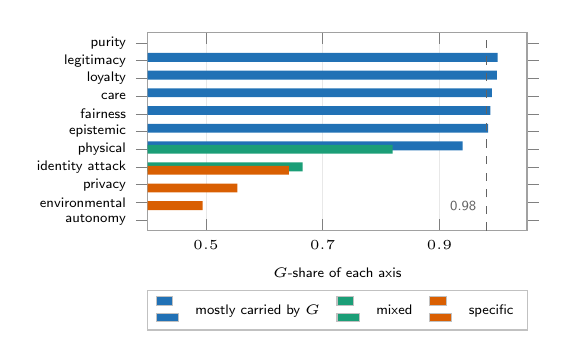
\begin{tikzpicture}
\begin{axis}[
  xbar, bar width=3.2pt,
  width=6.4cm, height=4.1cm,
  xmin=0.40, xmax=1.05, xtick={0.5,0.7,0.9},
  symbolic y coords={autonomy, environmental, privacy, identity attack,
    physical, epistemic, fairness, care, loyalty, legitimacy, purity},
  ytick={autonomy, environmental, privacy, identity attack,
    physical, epistemic, fairness, care, loyalty, legitimacy, purity},
  y tick label style={font=\tiny},
  x tick label style={font=\tiny},
  xlabel={\tiny $G$-share of each axis},
  axis line style={cbgray!60},
  xmajorgrids, grid style={cbgray!15, very thin},
  legend style={at={(0.5,-0.30)}, anchor=north, legend columns=3,
    font=\tiny, draw=cbgray!40, fill=white, column sep=4pt},
  legend cell align=left,
  enlarge y limits=0.06,
]
\addplot[xbar, fill=cbblue, draw=none] coordinates {
  (0.9997,purity) (0.9986,legitimacy) (0.9900,loyalty)
  (0.9873,care) (0.9836,fairness) (0.9396,epistemic)};
\addlegendentry{mostly carried by $G$}
\addplot[xbar, fill=cbteal, draw=none] coordinates {
  (0.8197,physical) (0.6658,identity attack)};
\addlegendentry{mixed}
\addplot[xbar, fill=cborange, draw=none] coordinates {
  (0.6421,privacy) (0.5538,environmental) (0.4945,autonomy)};
\addlegendentry{specific}
\draw[dashed, cbgray] ({axis cs:0.98,autonomy}|-{rel axis cs:0,0})
  -- ({axis cs:0.98,autonomy}|-{rel axis cs:0,1})
  node[pos=0.05, anchor=south east, font=\tiny, text=cbgray] {0.98};
\end{axis}
\end{tikzpicture}
\end{column}
\begin{column}{0.46\textwidth}
\begin{block}{\small Consequence for Secure AI}
\small A scalar \emph{harm} score is \gold{measured, not argued}, to be mostly $G$ --- and a scalar robustness score inherits the collapse by construction. The vulnerability structure lives in the \hi{surviving specific axes}.
\end{block}
\smallskip
{\footnotesize And the \hi{judge panel's own 31$\times$7 matrix replicates it}: PC1 = \gold{54\%}, the only component surviving parallel analysis; \hi{physical} fully specific there too; financial/identity diverge across instantiations.}
\end{column}
\end{columns}
\vfill
{\tiny Bifactor: learned-encoder instantiation (\texttt{xbse}), 12$\times$12 gate at margin 0.05; \texttt{identity\_attack} divergence recorded, not adjudicated. Panel FA: Horn's parallel analysis, $n{=}31$; per-judge FAs agree --- one factor in all six models (PC1 0.51--0.60), Tucker congruence 0.989--0.999 vs consensus. July 2026.}
\end{frame}

% ---------------------------------------------------------------
\begin{frame}{Implications for Secure AI deployment}
\begin{itemize}
  \item \hi{Where to look}: attacks that repackage the same facts with different \gold{salience} (euphemistic minimization).
  \item \hi{Prompt-level defenses are bounded}: explicit warnings recover only $\sim$38\% --- a ceiling co-occurring with universal overconfidence (ECE 0.19--0.42).
  \item \hi{Ask the right question}: ``\emph{which} vulnerabilities matter for our use case?'' --- not ``what's the robustness score?''
  \item \hi{Hardening target}: the fact-extraction front-end, since downstream kernels inherit its failures.
\end{itemize}
\end{frame}

% ---------------------------------------------------------------
\begin{frame}{The larger program: \emph{philosophy engineering}}
{\small This paper is one instance of a method: take a construct usually settled by \hi{argument} --- \emph{what is a harm? has this judgment been manipulated?} --- and build it into an \gold{instrument} you can measure, falsify, and harden.\par}
\vfill
\begin{columns}[T]
\begin{column}{0.53\textwidth}
\textbf{\small What makes it engineering, not rhetoric}
\begin{itemize}
  \item \small A \hi{space}, not a slogan: judgments are points, manipulation is \hi{displacement}, robustness is \hi{invariance}.
  \item \small \hi{Pre-registration} + \hi{admission gates that retract}: this talk's own bifactor test \emph{failed} its $P1$; a channel rescue was \emph{refuted}. Claims that do not transfer are \gold{publicly demoted}.
\end{itemize}
\end{column}
\begin{column}{0.43\textwidth}
\begin{block}{\small The conjecture behind the program {\scriptsize(not tested here)}}
\small Normative and aesthetic structure is \gold{geometric} --- it lives in \hi{compressibility} and \hi{coarse-graining under an observer}.\\[3pt]
One instrument, many domains: \hi{harm} today; \hi{aesthetics, law, cognition} on the same frame.
\end{block}
\end{column}
\end{columns}
\vfill
{\scriptsize A philosophical claim you can \gold{build, measure, and be proven wrong about} outranks one you can only defend.}
\end{frame}

% ---------------------------------------------------------------
\begin{frame}{Takeaways}
\begin{block}{Four takeaways}
\begin{enumerate}
  \item Vulnerabilities are \gold{selective} --- salience manipulation is the surface.
  \item Robustness profiles are \gold{dissociable} --- and a single score is now \emph{measured} to be mostly general valence.
  \item The exploit is \gold{end-to-end} --- it flips scalar scores \emph{and} typed verdicts.
  \item It is \gold{defensible} --- class averaging halves natural-paraphrase drift; adversarial-at-scale is the registered open item.
\end{enumerate}
\end{block}
\vfill
{\scriptsize Reproducible: \texttt{pip install agi-hpc} (tag \texttt{bds2026-v2}) \textperiodcentered\ \texttt{moral-spectrum-analyzer} \textperiodcentered\ \texttt{xbse} \textperiodcentered\ kernel: ErisML / DEME v3 \textperiodcentered\ five tracks, $\sim$8{,}000 calls under \$50/day (Kaggle); validation panel on the open NRP managed LLM API.}
\end{frame}

% ---------------------------------------------------------------
{\setbeamertemplate{footline}{}
\begin{frame}[plain]
\centering

\includegraphics[height=2.2cm]{atlas_mark_light.pdf}\\[8pt]
{\Large\textcolor{cbblue}{\textbf{Thank you}}}\\[4pt]
{\normalsize Andrew H. Bond \quad\textperiodcentered\quad \texttt{andrew.bond@sjsu.edu}}\\[2pt]
{\small Selective Invariance Violations in LLM Moral Judgment}\\
{\small IEEE BigDataService 2026 --- Secure AI}\\[6pt]
{\footnotesize Questions?}
\end{frame}}

% ================= BACKUP =======================================
\appendix

\begin{frame}{Backup --- grounding: 7-D harm space $\rightarrow$ DEME v3 9-D vector}
\centering
\small
\begin{tabular}{@{}lll@{}}
\toprule
\textbf{Harm dim.} & \textbf{DEME v3 axis} & \textbf{Mapping}\\
\midrule
physical & physical harm & direct\\
autonomy & autonomy / consent & direct\\
trust & legitimacy / trust & direct\\
social & societal / environmental & direct\\
financial & fairness / equity & partial\\
emotional & virtue / care & partial\\
identity & privacy / standing & partial\\
--- & rights, epistemic quality & not scored\\
\bottomrule
\end{tabular}
\vfill
{\small The evaluation pipeline is the \hi{measurement front-end}; the ErisML compiler's \hi{DEME bridge} is the downstream decision kernel (\texttt{DEMEVerdict}).}
\end{frame}

% ---------------------------------------------------------------
\begin{frame}{Backup --- the harm space is extensible \emph{and} falsifiable}
\textbf{Discovery loop}: residual analysis flags candidate missing dimensions $\rightarrow$ pre-registered admission gate.
\begin{itemize}
  \item Scorecard: 3 flagged $\rightarrow$ \gold{1 validated} (\texttt{identity\_attack}), \gold{1 retracted} (threat), \gold{1 declined} (sexual content $\rightarrow$ policy channel); a registered rescue of the \texttt{rights} channel \gold{refuted} (trained 0.509 vs null 0.512). \hi{The gate really rejects --- in both directions.}
  \item \texttt{identity\_attack}: cross-dataset held-out AUROC \gold{0.80} CI $[0.78, 0.83]$ ($+0.25$ over null, 2 corpora, $n=6400$) --- wired live as a \hi{10th channel}.
  \item Cross-lingual at scale: invariance index \gold{0.72--0.80} across es/ar/zh/hi/sw, \hi{harmful $\approx$ benign}.
\end{itemize}
\vfill
{\scriptsize Validated on the learned-encoder perception layer (\texttt{xbse}); native DEME re-run of the five tracks is the extended version. Post-camera-ready results, July 2026.}
\end{frame}

\end{document}
